\section{简易调试技术}\label{sec:简易调试技术}

{
\setbeamertemplate{frame footer}{https://nju-projectn.github.io/ics-pa-gitbook/ics2016/}
\begin{frame}[fragile]{调试公理}
    \begin{quote}
        \begin{itemize}
            \item The machine is always right.
            \begin{itemize}
                \item Corollary: If the program does not produce the desired output, it is the programmer's fault.
            \end{itemize}
            \emptyline
            \item Every line of untested code is always wrong.
            \begin{itemize}
                \item Corollary: Mistakes are likely to appear in the ``must-be-correct'' code.
            \end{itemize}
        \end{itemize}
        \emptyline
        \hspace*{\fill} --jyy
    \end{quote}
\end{frame}
}

\begin{frame}[fragile]{常用的调试技能}
    前面讲了 设置严格的编译选项 和 将输入输出重定向 用于辅助调试, 但并不是真正的调试.
    我们常用的调试技术有哪些呢?
    \begin{itemize}[<+- | alert@+>]
        \item 输出调试 (相信大家都用过了)
        \item 设置断点 (在特定的地方停下来)
        \item 单步执行 (一步步看)
    \end{itemize}
\end{frame}

\begin{frame}[fragile]{手动输出调试(可能是错误示范)}
    \begin{itemize}[<+- | alert@+>]
        \item 不知道我的 bug 代码在干嘛, 看一看不就好了!
        \item (凭感觉)在可能出错的地方加上\texttt{printf()}或\texttt{cout}
        \item (凭感觉)输出有关的变量
        \item 没感觉怎么办?
        \item 加很多\texttt{printf()}
        \item -> 眼花缭乱的输出信息 + 调完还要删的\texttt{printf()}
        \item 改进?
    \end{itemize}
\end{frame}

\begin{frame}[fragile]{手动设置断点和单步调试(可能是错误示范)}
    \begin{itemize}[<+- | alert@+>]
        \item 不知道我的代码会不会走到一个分支, 停一下不就好了!
        \item 在想停的地方加上\texttt{getchar();}
        \item 在每个语句下都加个\texttt{getchar();}就可以单步执行了
        \item -> 非常麻烦 + 破坏输入格式 + 单步执行也难以获取有用信息
        \item 改进?
    \end{itemize}
\end{frame}

\begin{frame}[fragile]{设置断点}
    下载 \href{http://problemoverflow.top/download/function\_array.c}{function\_array.c}
    并将代码添加到一个CLion工程中.
    如果使用gcc编译, 需要添加编译选项 \texttt{-g -Og}
    \begin{itemize}[<+- | alert@+>]
        \item 我们希望程序执行到\texttt{main()}函数时停下
        \item 单击第20行行号右边空白, 产生一个红点 (gdb: \textbf{b}reak)
        \item Shift + F9 或单击调试的图标开始调试
        \begin{figure}[ht!]
            \centering
            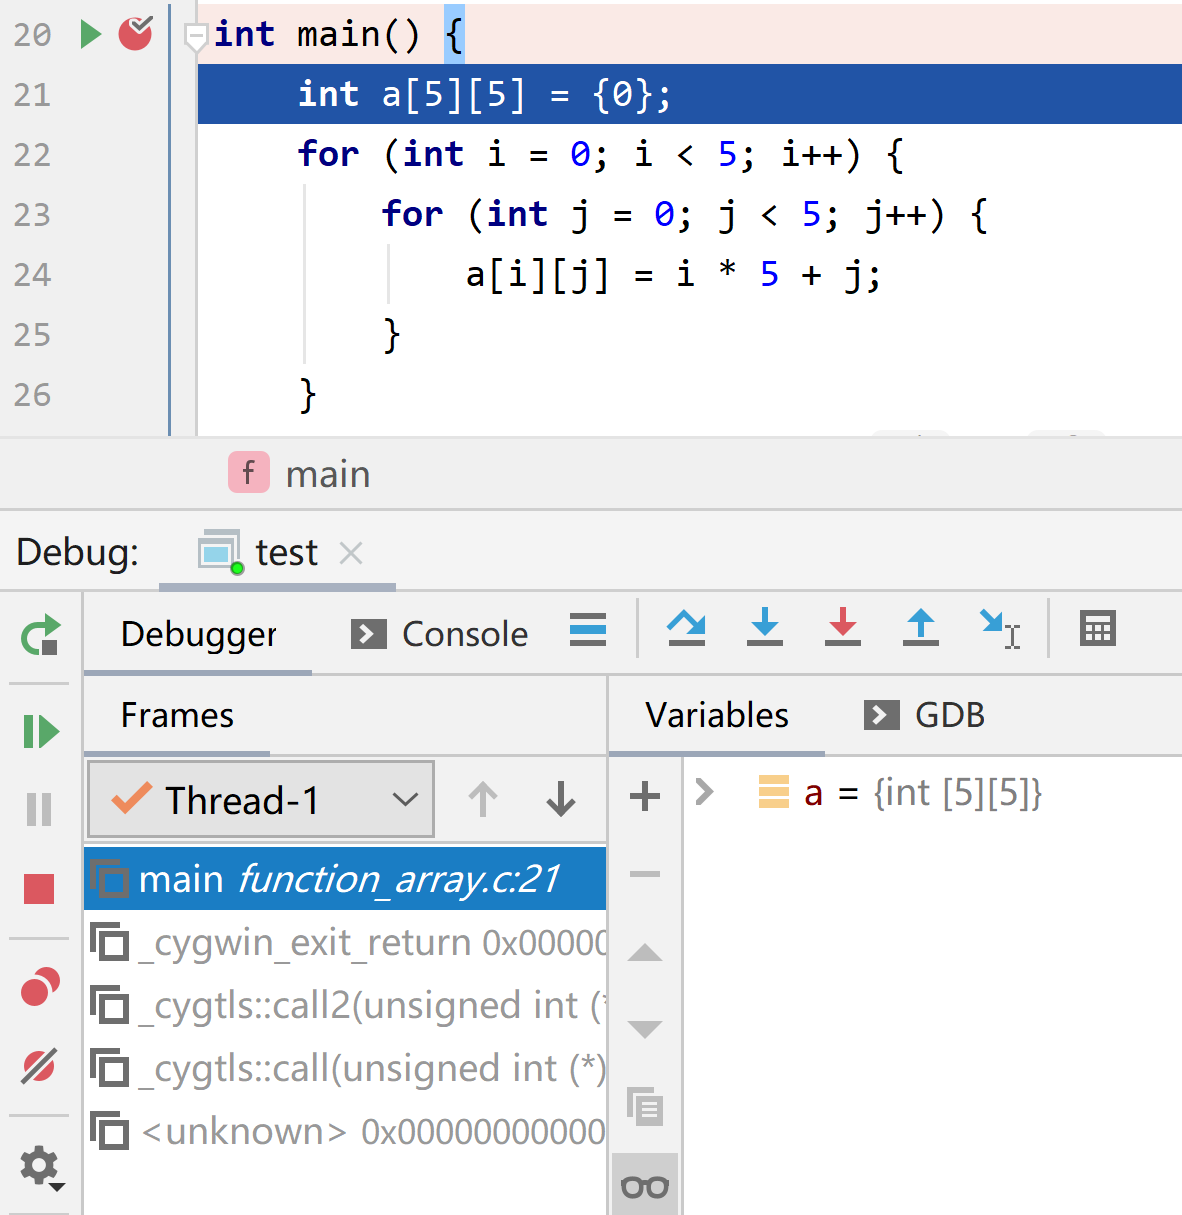
\includegraphics[width=50mm]{figs/clion_b_main.png}
            \caption{在main函数设置断点}
        \end{figure}
    \end{itemize}
\end{frame}

\begin{frame}[fragile]{查看变量信息}
    双击调试窗口Variables的空白处或点击 + 号, 输入你想观察的表达式 (gdb: \textbf{p}rint)
    \begin{figure}[ht!]
        \centering
        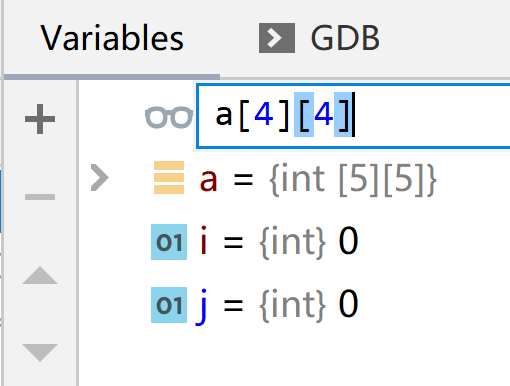
\includegraphics[height=25mm]{figs/clion_new_watch.png}
        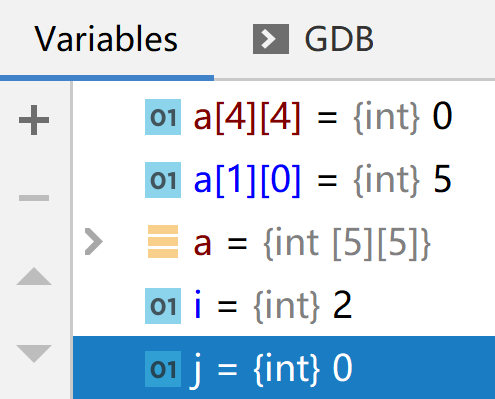
\includegraphics[height=25mm]{figs/clion_new_watch2.png}
        \caption{添加表达式}
    \end{figure}
\end{frame}

\begin{frame}[fragile]{单步执行}
    我们希望程序每次运行一行C语言代码, 便于观察执行那一步时的状态
    \begin{figure}[ht!]
        \centering
        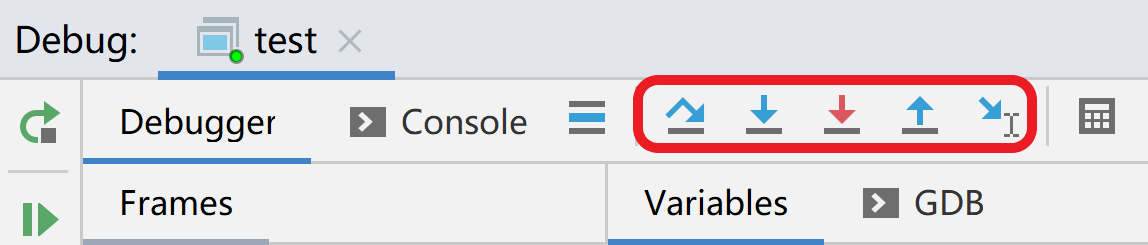
\includegraphics[width=50mm]{figs/clion_step_buttons.png}
        \caption{CLion调试单步执行按钮}
    \end{figure}
    从左到右依次的功能:
    \begin{itemize}[<+- | alert@+>]
        \item Step Over (F8, gdb: \textbf{n}ext): 执行一行C语言语句,  如果该行有函数调用, 函数将被执行完 (不单步进入函数体)
        \item Step Into (F7, gdb: \textbf{s}tep): 同上, 不同之处为会进入函数体
        \item Force Step Into: 同上, 不同之处为会进入标准库函数
        \item Step Out (Shift + F8, gdb: \textbf{fin}ish): 将当前的函数执行至结束
        \item Run to Cursor (Alt + F9): 执行到鼠标指针的位置
    \end{itemize}
\end{frame}

\begin{frame}[fragile]{添加监视点}
    我们希望程序能在某些条件满足的情况下停下, 比如变量被修改, 等于某个值, 大于某个值, 小于另一个变量等等
    \begin{itemize}[<+- | alert@+>]
        \item 先使用查看变量信息的方法添加你感兴趣的表达式
        \item 在该表达式上右键 - Add Watchpoint (gdb: watch)
        \item 查看监视点 (gdb: info watchpoints 或 info breakpoints)
        \begin{figure}[ht!]
            \centering
            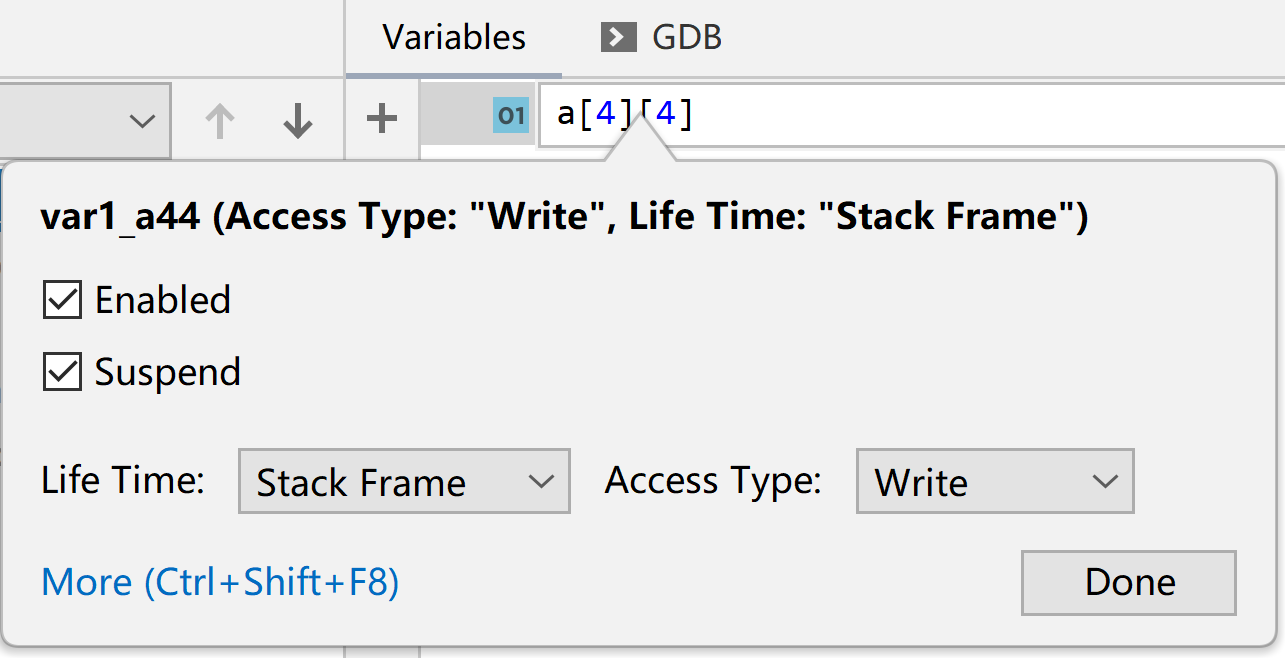
\includegraphics[height=25mm]{figs/clion_watchpoint.png}
            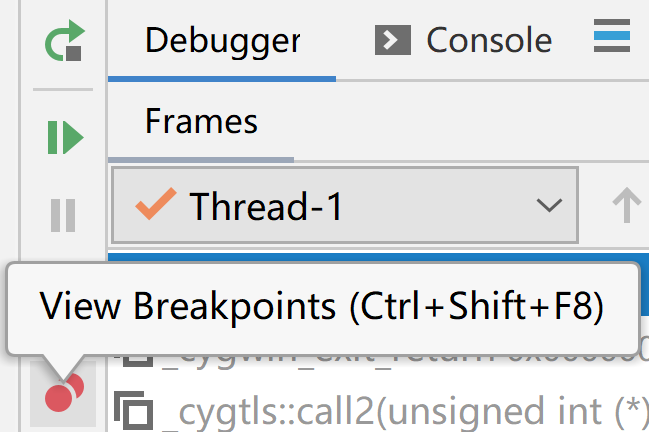
\includegraphics[height=25mm]{figs/clion_info_watchpoint.png}
            \caption{CLion添加和查看监视点}
        \end{figure}
    \end{itemize}
\end{frame}

\begin{frame}[fragile]{查看调用链}
    \texttt{main()}调用了\texttt{printSumArray()}.
    而执行到\texttt{printSumArray()}时, 我们希望查看\texttt{main()}的变量状态.
    \begin{itemize}[<+- | alert@+>]
        \item 每个函数调用是一个栈帧, CLion的Frames窗口有栈帧信息 (gdb: \textbf{b}ack\textbf{t}race)
        \item 点击其他的栈帧可以切换 (gdb: \textbf{f}rame)
        \begin{figure}[ht!]
            \centering
            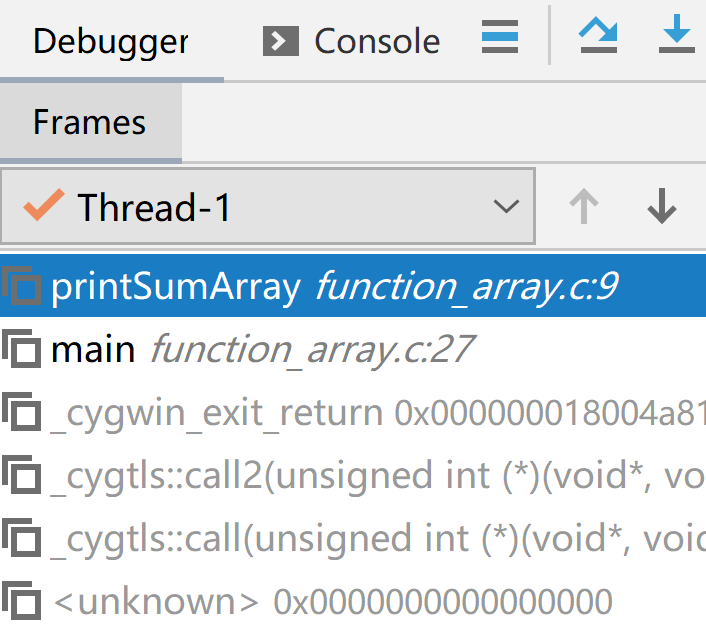
\includegraphics[width=40mm]{figs/clion_frame.png}
            \caption{CLion查看栈帧链}
        \end{figure}
    \end{itemize}
\end{frame}

\begin{frame}[fragile]{使用GDB}
    打开CLion调试的GDB窗口, 或使用命令行 \textbf{gdb ./main.exe}

    \begin{table}[]
        \begin{tabular}{|l|l|}
            \hline
            \textbf{行为} & \textbf{命令} \\ \hline
            设置断点在\texttt{main()} & \texttt{b main} \\ \hline
            设置断点在第八行 & \texttt{b 8} \\ \hline
            运行程序 & \texttt{r} \\ \hline
            继续执行 & \texttt{c} \\ \hline
            查看变量a[4][4] & \texttt{p a[4][4]} \\ \hline
            单步不进入函数执行3行 & \texttt{n 3} \\ \hline
            单步进入函数执行1行 & \texttt{s} \\ \hline
            执行当前函数至返回 & \texttt{fin} \\ \hline
            当a[4][4]的值改变时停下 & \texttt{watch a[4][4]} \\ \hline
            当a[3][3]的值不等于0时停下 & \texttt{watch a[3][3] != 0} \\ \hline
            查看断点 & \texttt{info breakpoints} \\ \hline
            查看栈帧链 & \texttt{bt} \\ \hline
            选择栈帧\#1 & \texttt{f 1} \\ \hline
        \end{tabular}
        \caption{GDB常用命令一览表}
    \end{table}
\end{frame}